\begin{exercise}
      {ID-416763be84d77206045d05edc5ffde53806c7e83}
      {Kreisringe}
  \ifproblem\problem
    \begin{enumerate}[a)]
      \item Ein Kreisring besitzt einen inneren Radius von \sicm{5} und eine
            Fläche von \sicmm{12}. Wie groß ist der äußere Radius $r_{a}$?
      \item Ein Kreisring besitzt eine Fläche von \sicmm{40}. Die Summe
            seiner Radien ergibt \sicm{15}. Wie groß ist der Innenradius
            $r_{i}$?
      \item Ein Kreisring besitzt einen Außenradius von \sicm{12}. Er soll
            die gleiche Fläche wie sein Innenkreis haben. Wie groß ist der
            Innenradius $r_{i}$?
    \end{enumerate}
  \fi
  \ifoutline\outline
    Die Lösungen erhält man, indem man die Gleichung zur Bestimmung des
    Flächeninhalts von Kreisringen $A=\pi r_a^2-\pi r_i^2$ nach den
    gesuchten Größen auflöst:\par
    \begingroup
      \dimen1=4.5cm%
      \begin{minipage}{\dimen1}%
        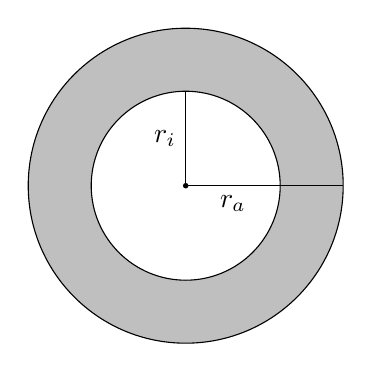
\begin{tikzpicture}%
          \draw[line width=8mm, draw=black!25!white]
               (0, 0) circle[radius=1.6cm];
          \draw (0, 0) circle[radius=1.2cm];
          \draw (0, 0) circle[radius=2.0cm];
          \fill[fill=black] (0, 0) circle[radius=1pt];
          \draw (0, 0) -- node[left]{$r_i$} +(90:1.2);
          \draw (0, 0) -- node[below, pos=0.3]{$r_a$} +(0:2.0);
        \end{tikzpicture}%
      \end{minipage}%
      \dimen2=\linewidth%
      \advance\dimen2 by -\dimen1%
      \begin{minipage}{\dimen2}%
        \setlength{\abovedisplayskip}{0pt}%
        \begin{equation*}
          \begin{split}
            \text{a)}&\quad
            A=\pi\cdot\left(r_a^2-r_i^2\right)
            \quad\Rightarrow\quad
            r_a=\sqrt{\frac{A}{\pi}+r_i^2}
            \\[2ex]
            \text{b)}&\quad
            r_a+r_i=s
            \quad\Rightarrow\quad
            r_a=s-r_i
            \\
            \text{~}&\quad
            A=\pi\cdot\left((s-r_i)^2-r_i^2\right)
            \quad\Rightarrow\quad
            r_i=\frac{s}{2}-\frac{A}{2\pi s}
            \\[2ex]
            \text{c)}&\quad
            r_i=\pi r_a^2-\pi r_i^2
            \quad\Rightarrow\quad
            0=r_i^2+\frac{1}{\pi}\cdot r_i-r_a^2
            \\
            \text{~}&\quad
            r_i=-\frac{1}{2\pi}+\sqrt{\frac{1}{4\pi^2}+r_a^2}
          \end{split}
        \end{equation*}
      \end{minipage}%
    \endgroup
  \fi
  \ifoutcome\outcome
    \begin{enumerate}[a)]
      \item Der Außenradius $r_a$ besitzt eine Länge von ca. \sicm{5.368}.
      \item Der Innenradius $r_i$ besitzt eine Länge von ca. \sicm{7.076}.
      \item Der Innenradius $r_i$ besitzt eine Länge von ca. \sicm{11.842}.
    \end{enumerate}
  \fi
\end{exercise}
